%==========================================================================
% BEGIN #5 - ESBOÇO DOS INTERFACES DO SISTEMA
% Descrição e caracterização das diversas interfaces requeridas pelos serviços do sistema, utilizando esboços (mockups) que revelem o aspeto pretendido para cada uma das interfaces a implementar.
%==========================================================================

\chapter{Esboço dos Interfaces do Sistema}

    Em primeiro lugar, criou-se um logótipo simples de modo a poder ser utilizado nas interfaces sem criar muita poluição visual. Consiste apenas numa peça de lego com o nome da empresa.

    \begin{figure}[h!]
        \centering
        \includegraphics[width=0.5\linewidth]{images/autobricklogo.png}
        \caption{Logótipo}
        \label{fig:Logo}
    \end{figure}

    Para além disto, escolheu-se uma palete de cores que serão utilizadas nas interfaces de forma a torná-las mais apelativas esteticamente.

        \begin{figure}[h!]
        \centering
        \includegraphics[width=0.8\linewidth, frame]{images/ColorPallete.png}
        \caption{Palete de cores}
        \label{fig:Palete de cores}
    \end{figure}

    Segue, assim, uma apresentação das principais interfaces.

    \clearpage
    \subsection{Interfaces de autenticação}
    
        \begin{figure}[h!]
            \centering
            \includegraphics[width=0.99\linewidth, frame]{images/Login Failed.pdf}
            \caption{Página de Login (com credenciais erradas) }
            \label{fig:Login}
        \end{figure}
    
        Esta é a página utilizada para iniciar sessão (ver requisito 2.2.2)

        \clearpage
        \begin{figure}[h!]
            \centering
            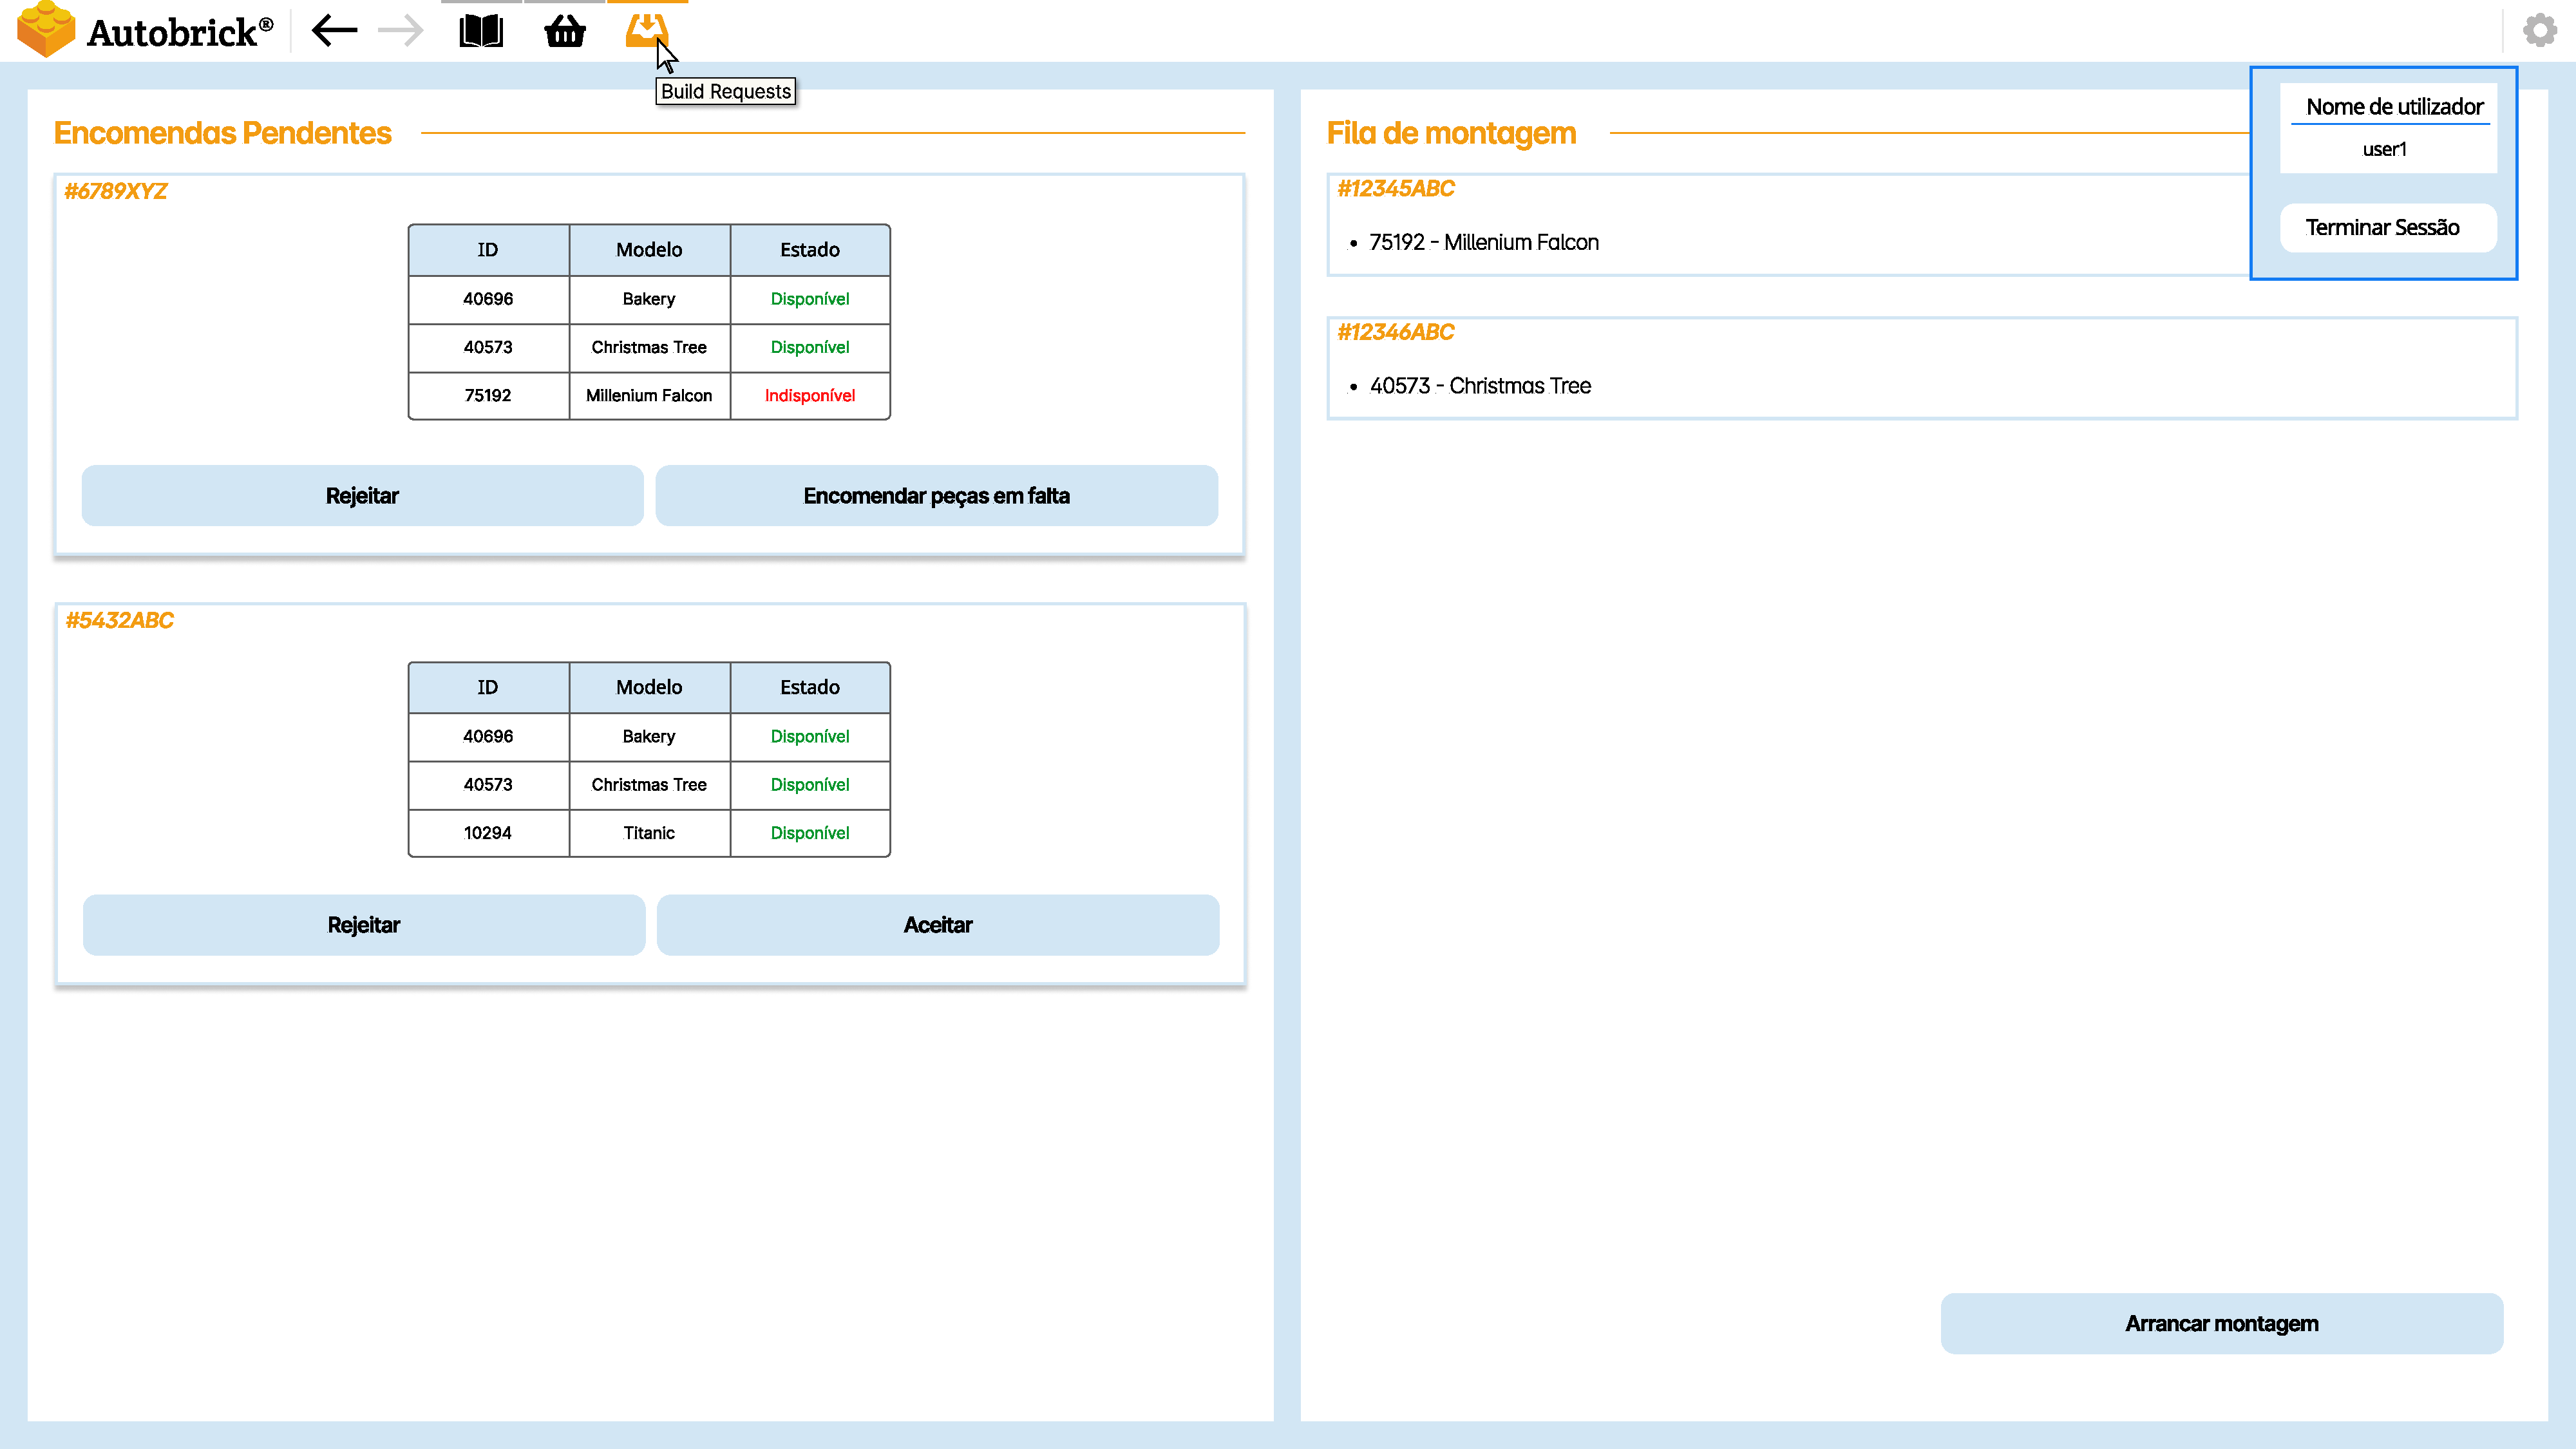
\includegraphics[width=0.99\linewidth, frame]{images/Settings.pdf}
            \caption{Página de encomendas após interação com botão de opções (engrenagem)}
            \label{fig:Settings}
        \end{figure}
        
        Quando o utilizador clica na engrenagem no canto superior direito da página, aparece um menu que lhe mostra o seu nome de utilizador (ver requisito 2.2.4) e um botão para terminar sessão (ver requisito 2.2.3).
    
        \clearpage
        \begin{figure}[h!]
            \centering
            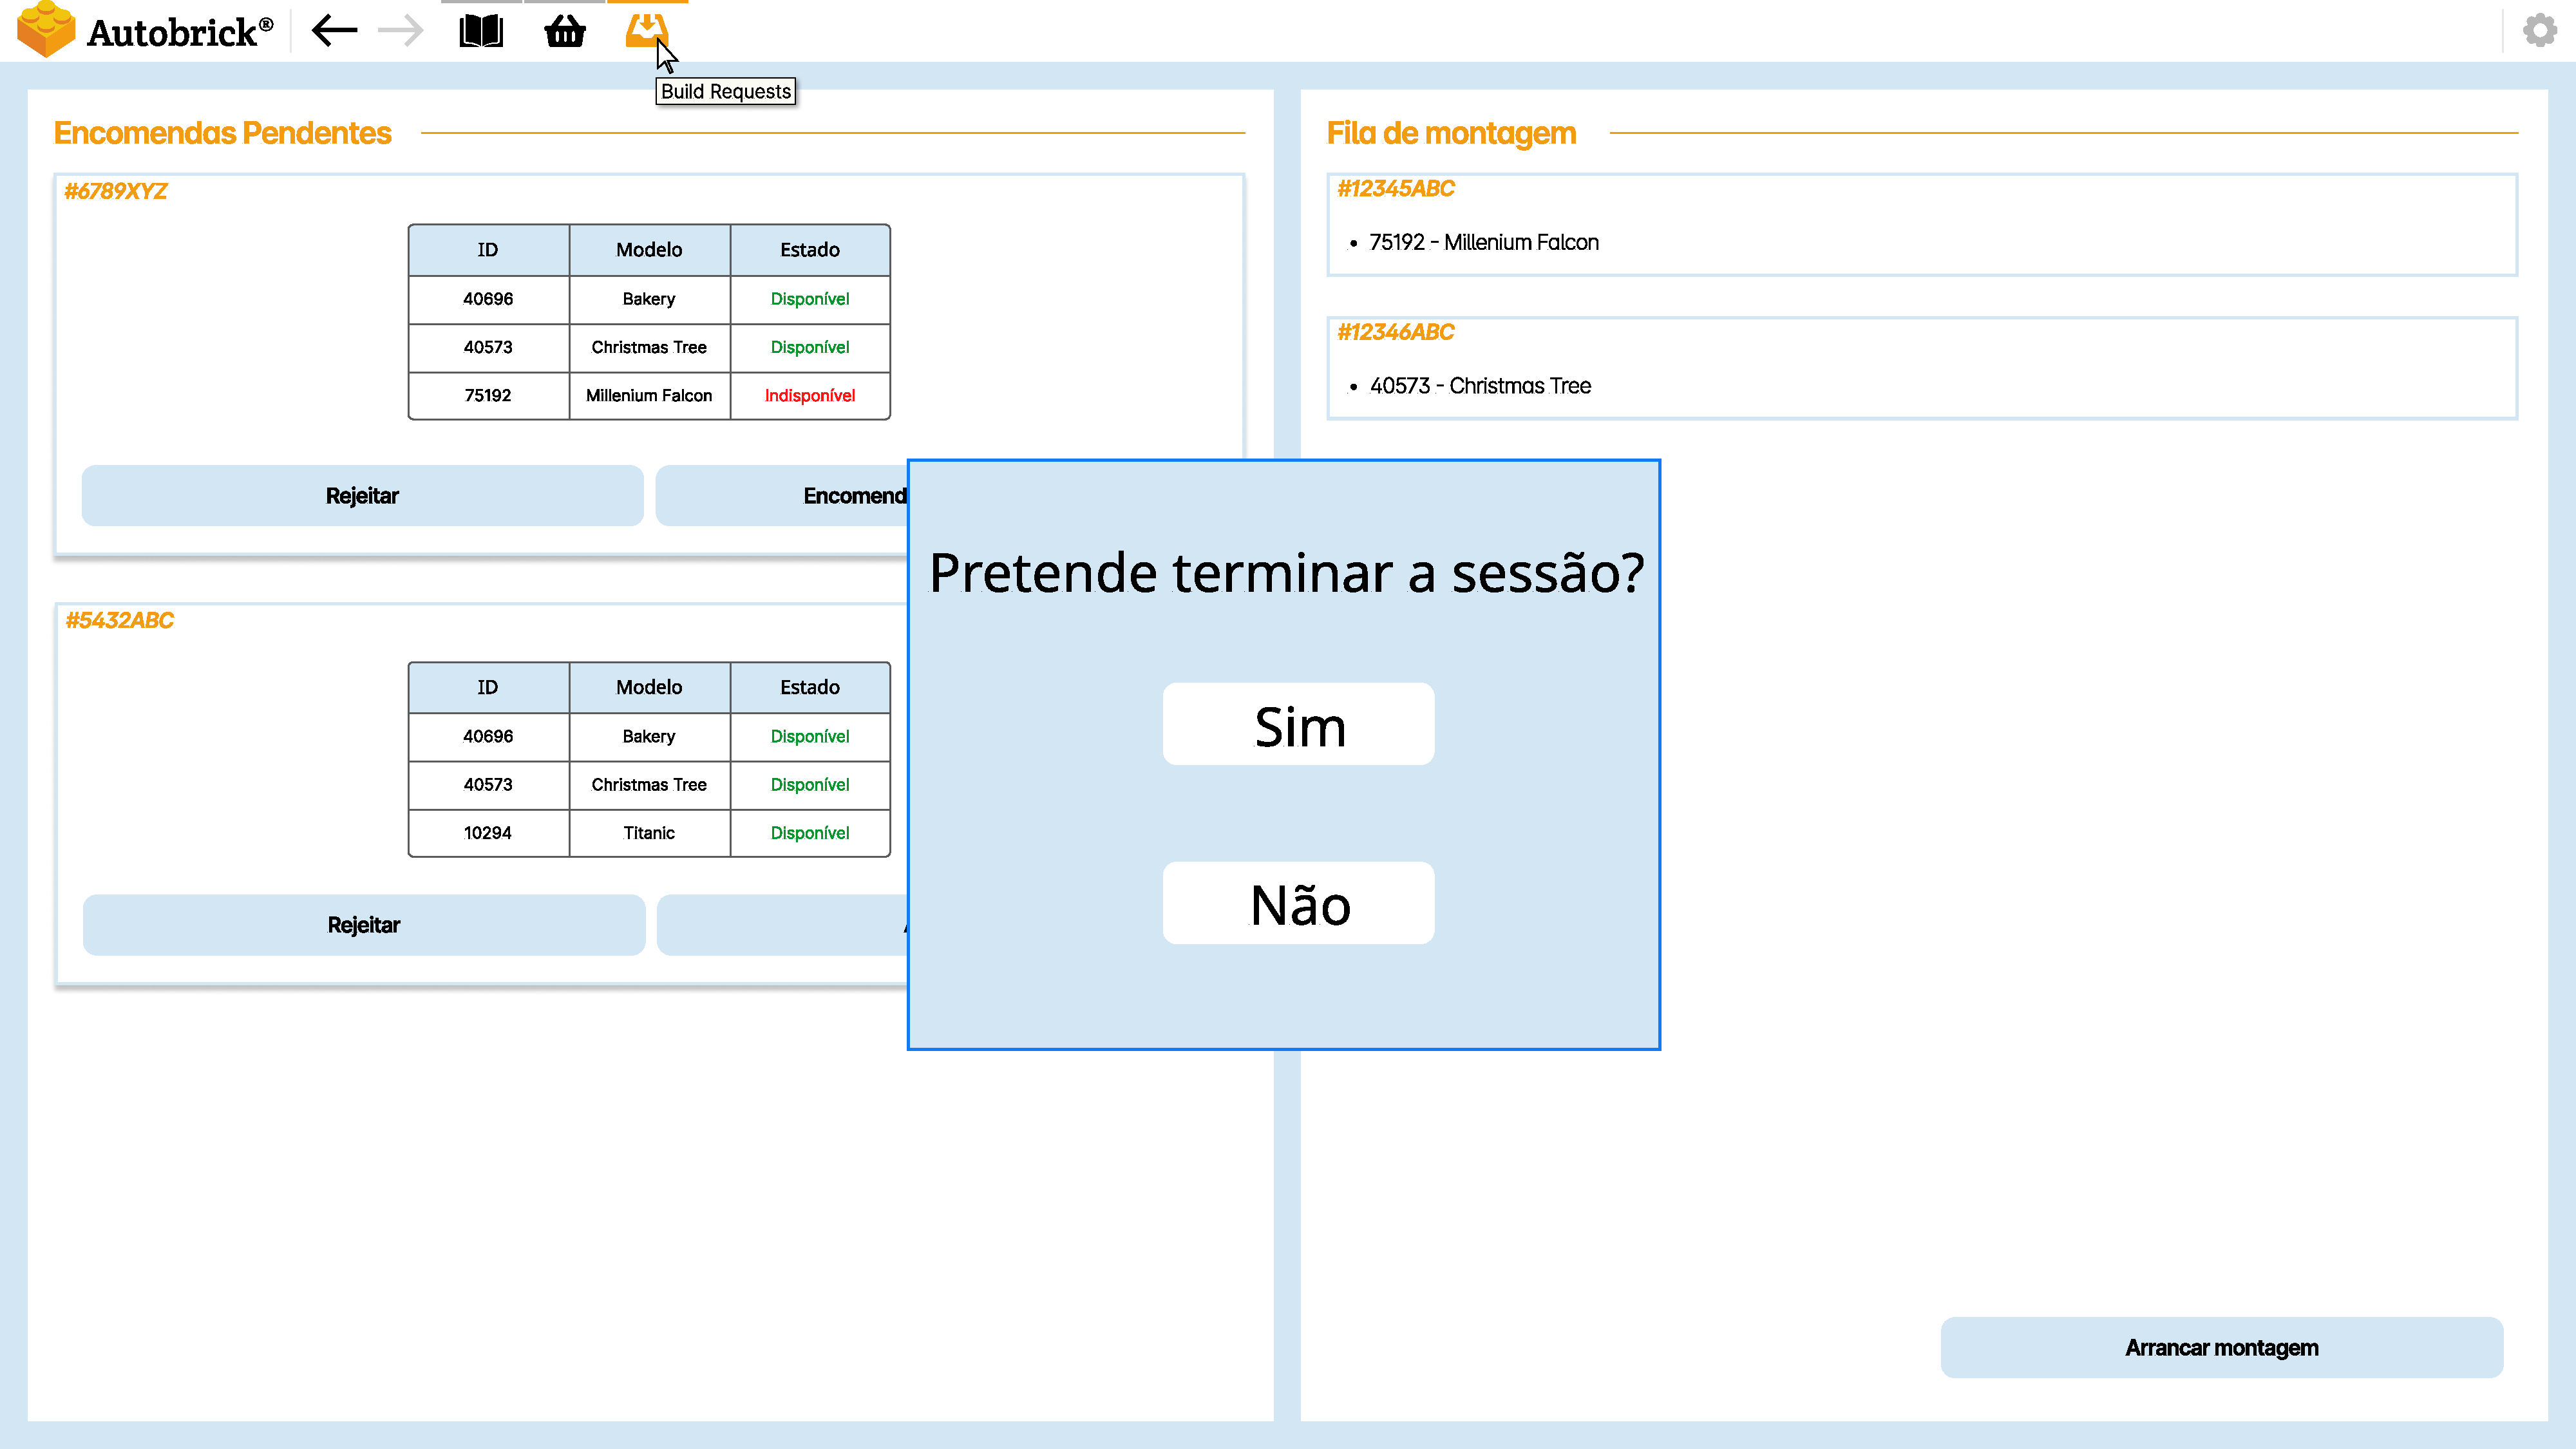
\includegraphics[width=0.99\linewidth, frame]{images/Logout.pdf}
            \caption{Página de encomendas após interação com botão de terminar sessão}
            \label{fig:Logout}
        \end{figure}
    
        Quando o utilizador carrega no botão de terminar sessão, o menu da Figura~\ref{fig:Logout} aparece para este confirmar a ação.
    
    \clearpage
    \subsection{Interfaces de Encomendas}

        \begin{figure}[h!]
            \centering
            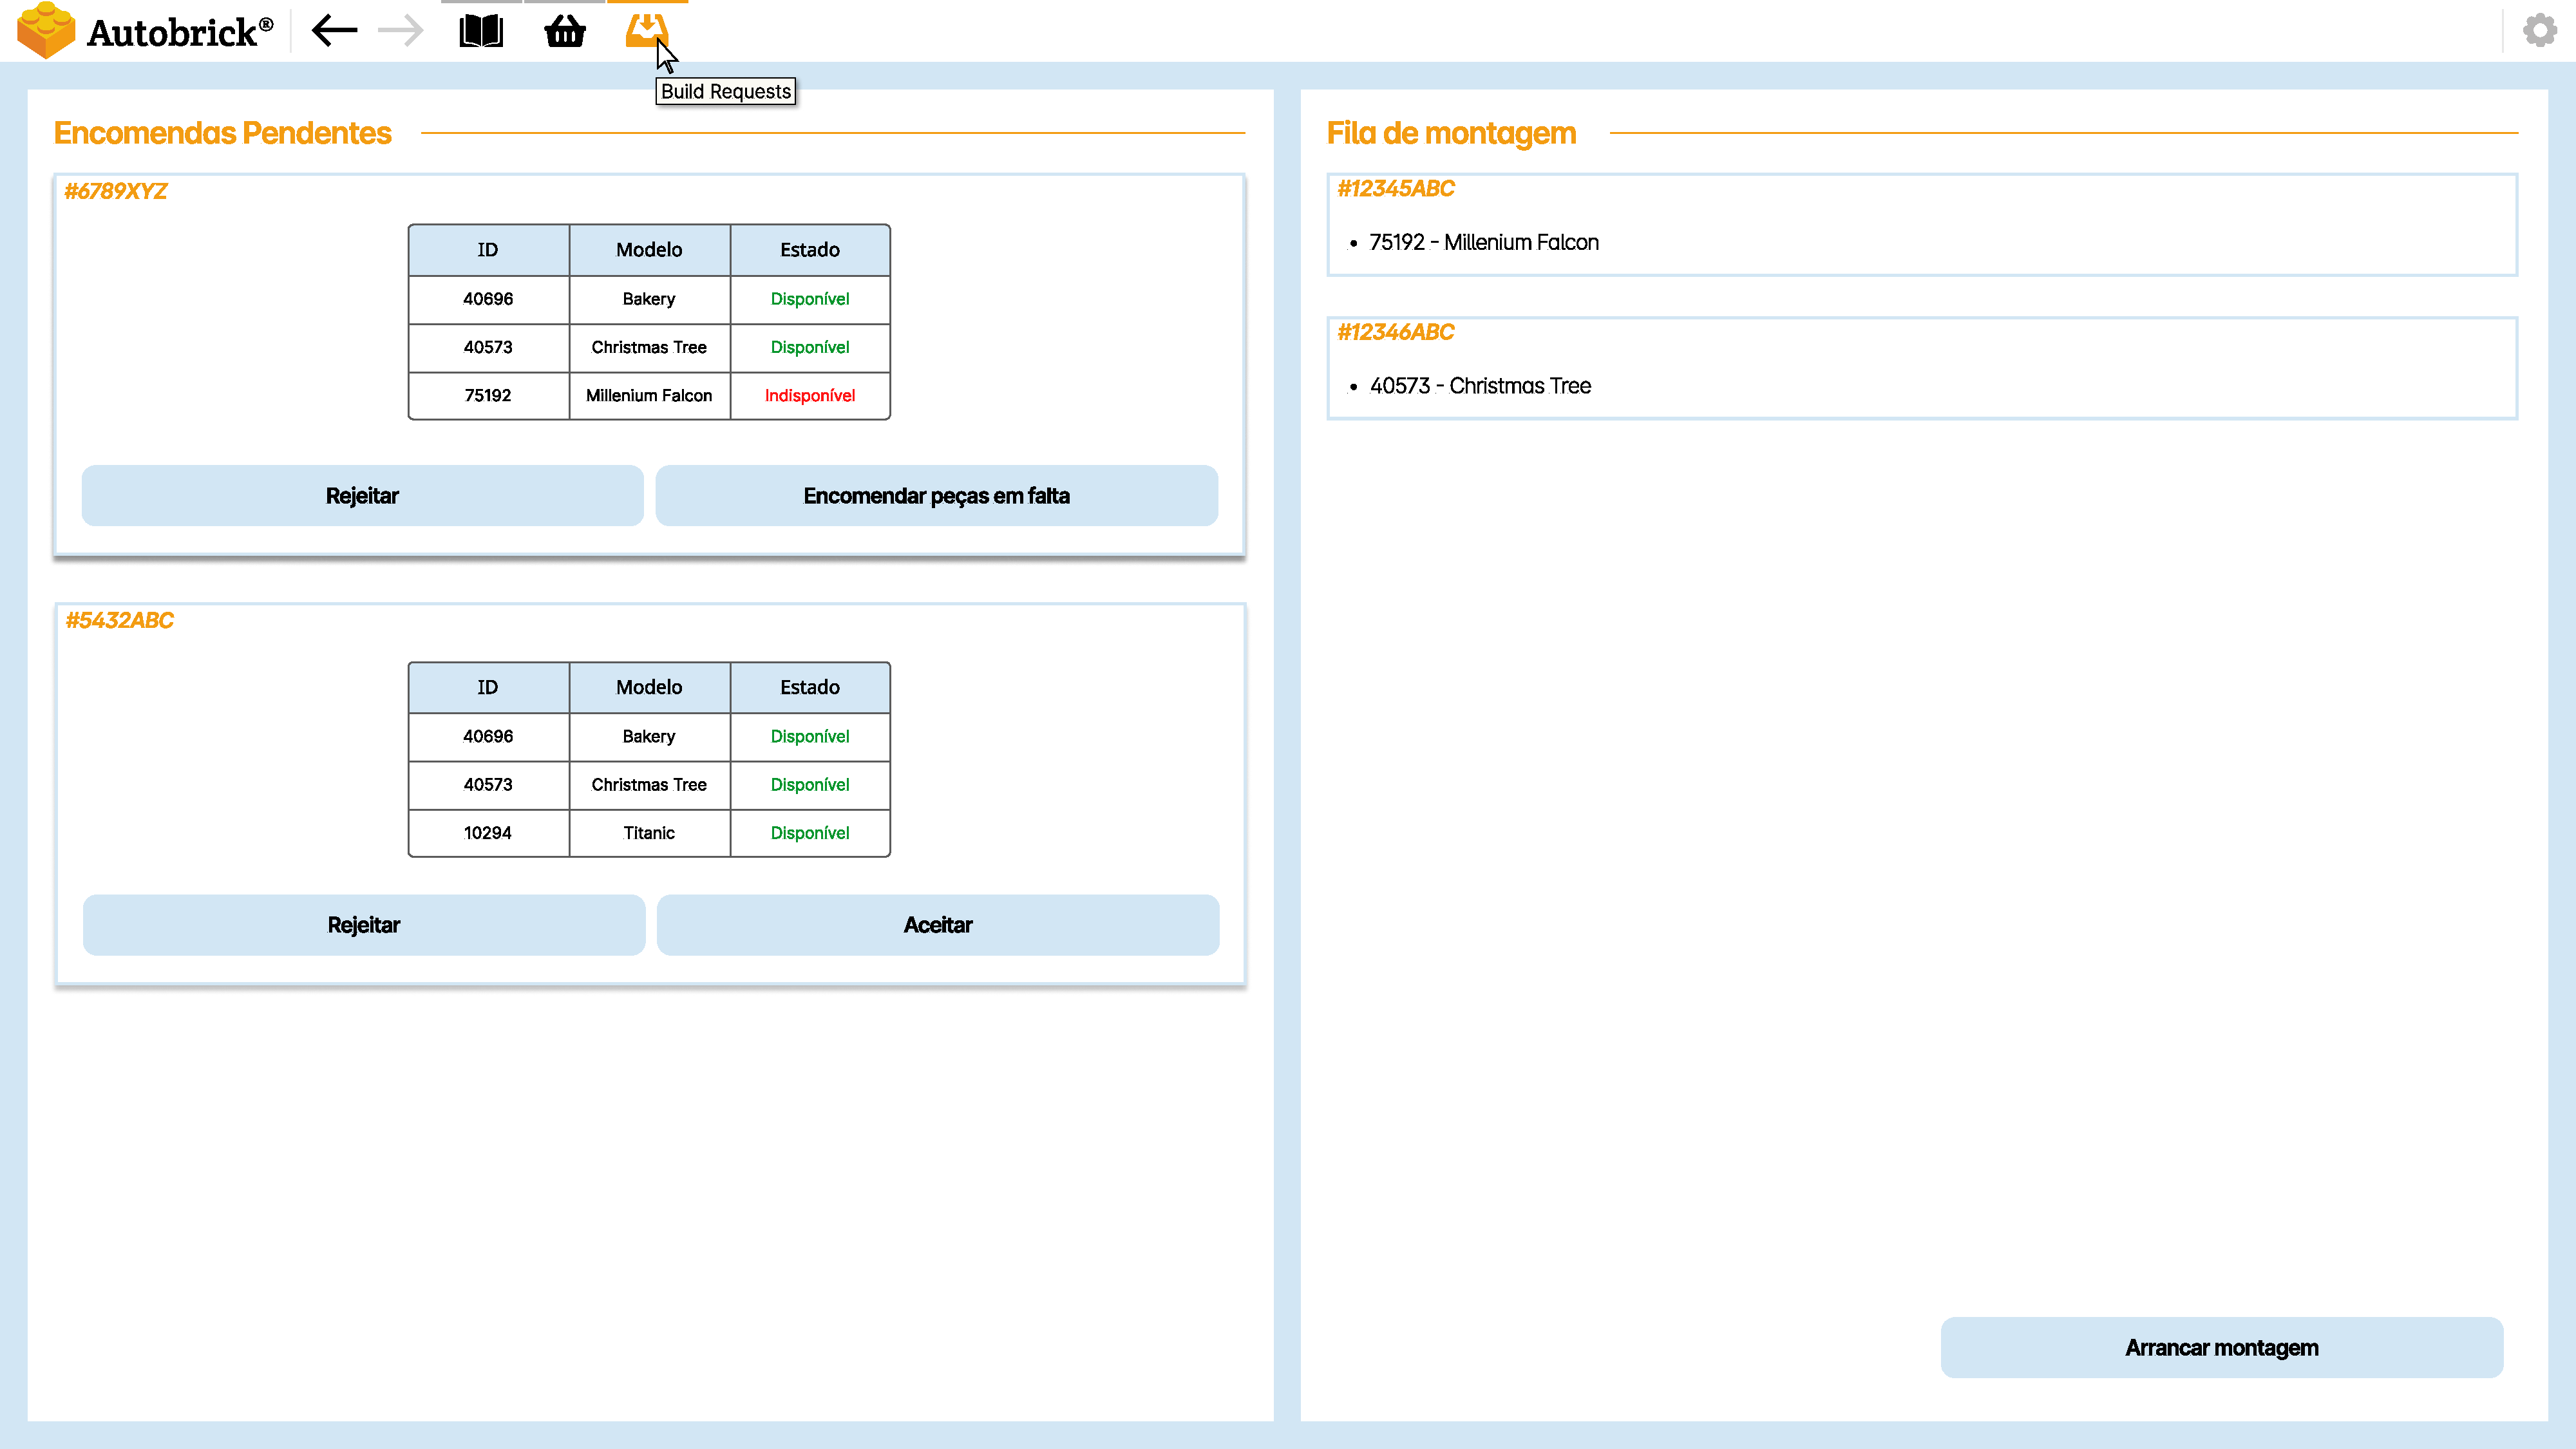
\includegraphics[width=0.85\linewidth, frame]{images/Requests.pdf}
            \caption{Página de encomendas}
            \label{fig:Encomendas}
        \end{figure}
    
        Esta é considerada a páginal principal da aplicação onde é possível iniciar a montagem da próxima encomenda na fila de montagem (ver use case 3.3.1.3), consultar encomendas pendentes (use case 3.3.1.1) bem como rejeitar ou aceitar as mesmas (ver use case 3.3.1.2). Para além disso é ainda possível encomendar as peças em falta para realizar um dado modelo (ver use case 3.3.1.2 e 3.3.2.2)
    
    
        \begin{figure}[h!]
            \centering
            \includegraphics[width=0.85\linewidth, frame]{images/Encomenda Automática.pdf}
            \caption{Página de encomendas após interação com botão de encomendar peças em falta}
            \label{fig:EncomendasAuto}
        \end{figure}
        
    \clearpage
    \subsection{Interfaces de Inventário}
    
        \begin{figure}[h!]
            \centering
            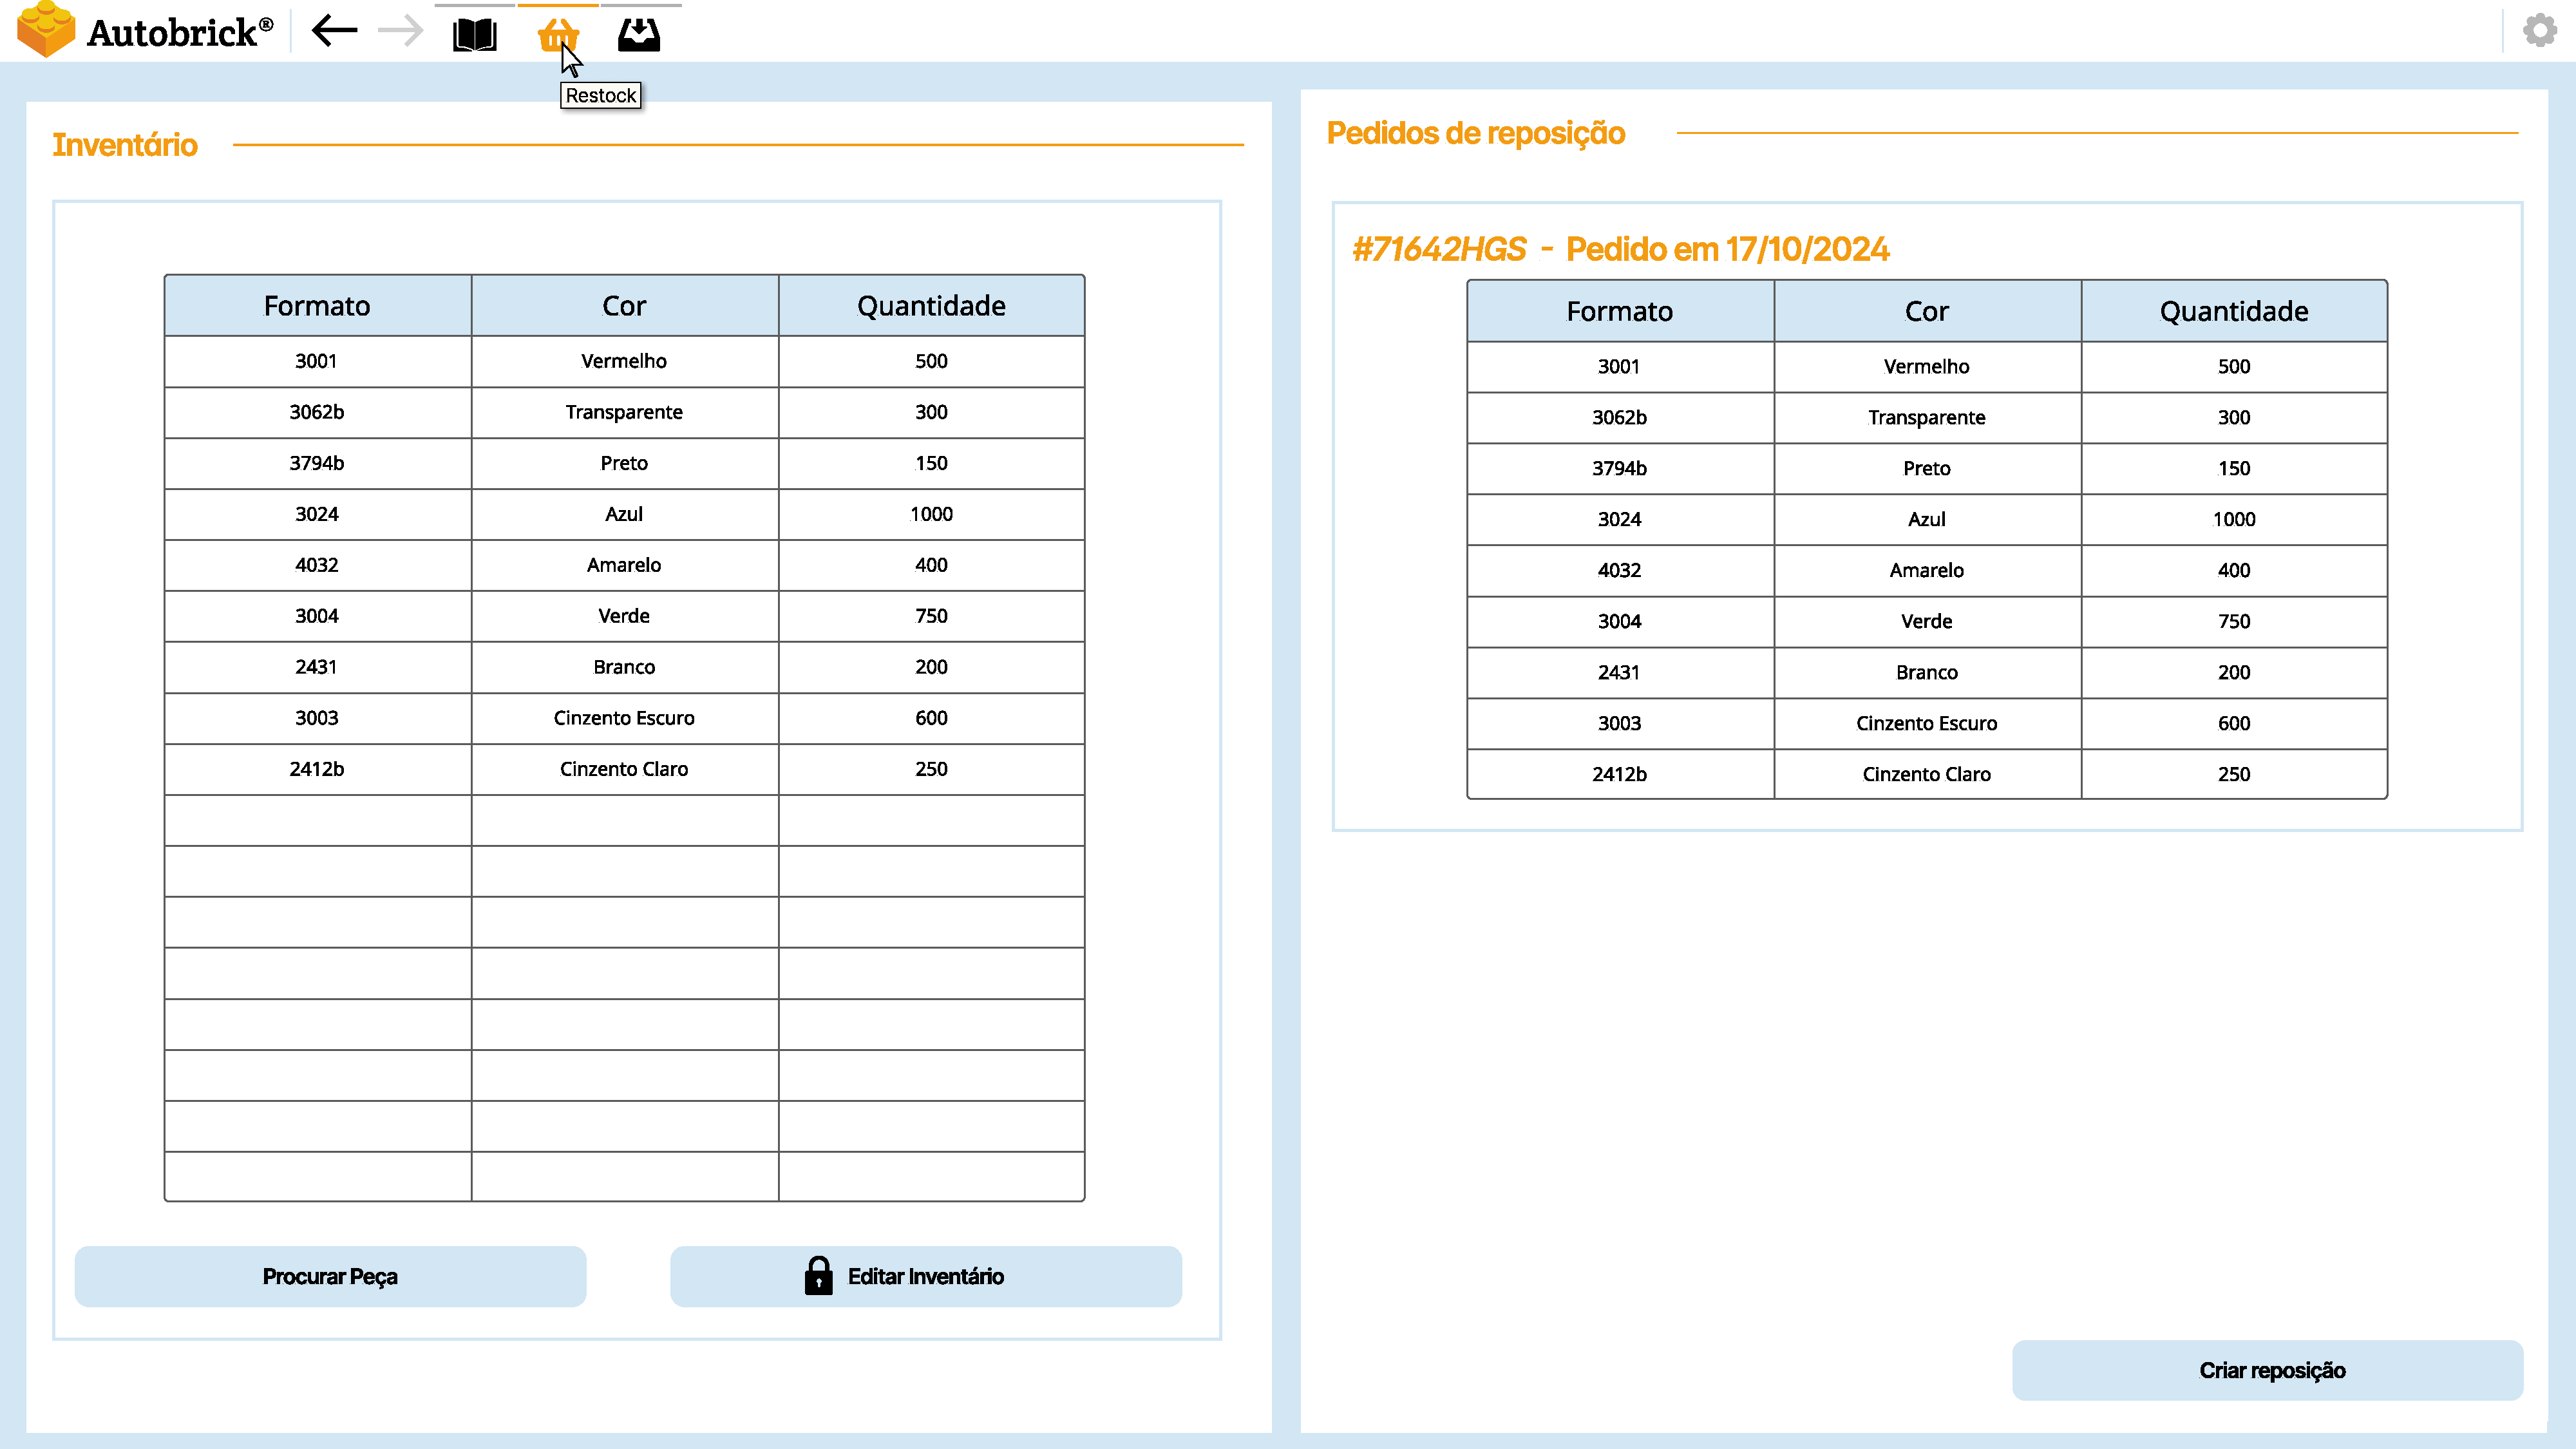
\includegraphics[width=0.99\linewidth, frame]{images/Restock I.pdf}
            \caption{Página de inventário}
            \label{fig:Inventário}
        \end{figure}
    
        Nesta página é possivel consultar o inventário de peças disponíveis (ver 2.4.1). Ainda nesta página é dada opção de fazer uma reposição manual (Figura~\ref{fig:Reposição})(ver use case 3.3.2.1) e é dada a possibilidade de editar a quantidade disponível de uma dada peça, caso esta opção seja selecionada o utilizador deve inserir a palavra passe de administrador (Figura~\ref{fig:EditarInv1}) e inserir os dados da peça alterar (Figura~\ref{fig:EditarInv2}) 
    
        \begin{figure}[h!]
            \centering
            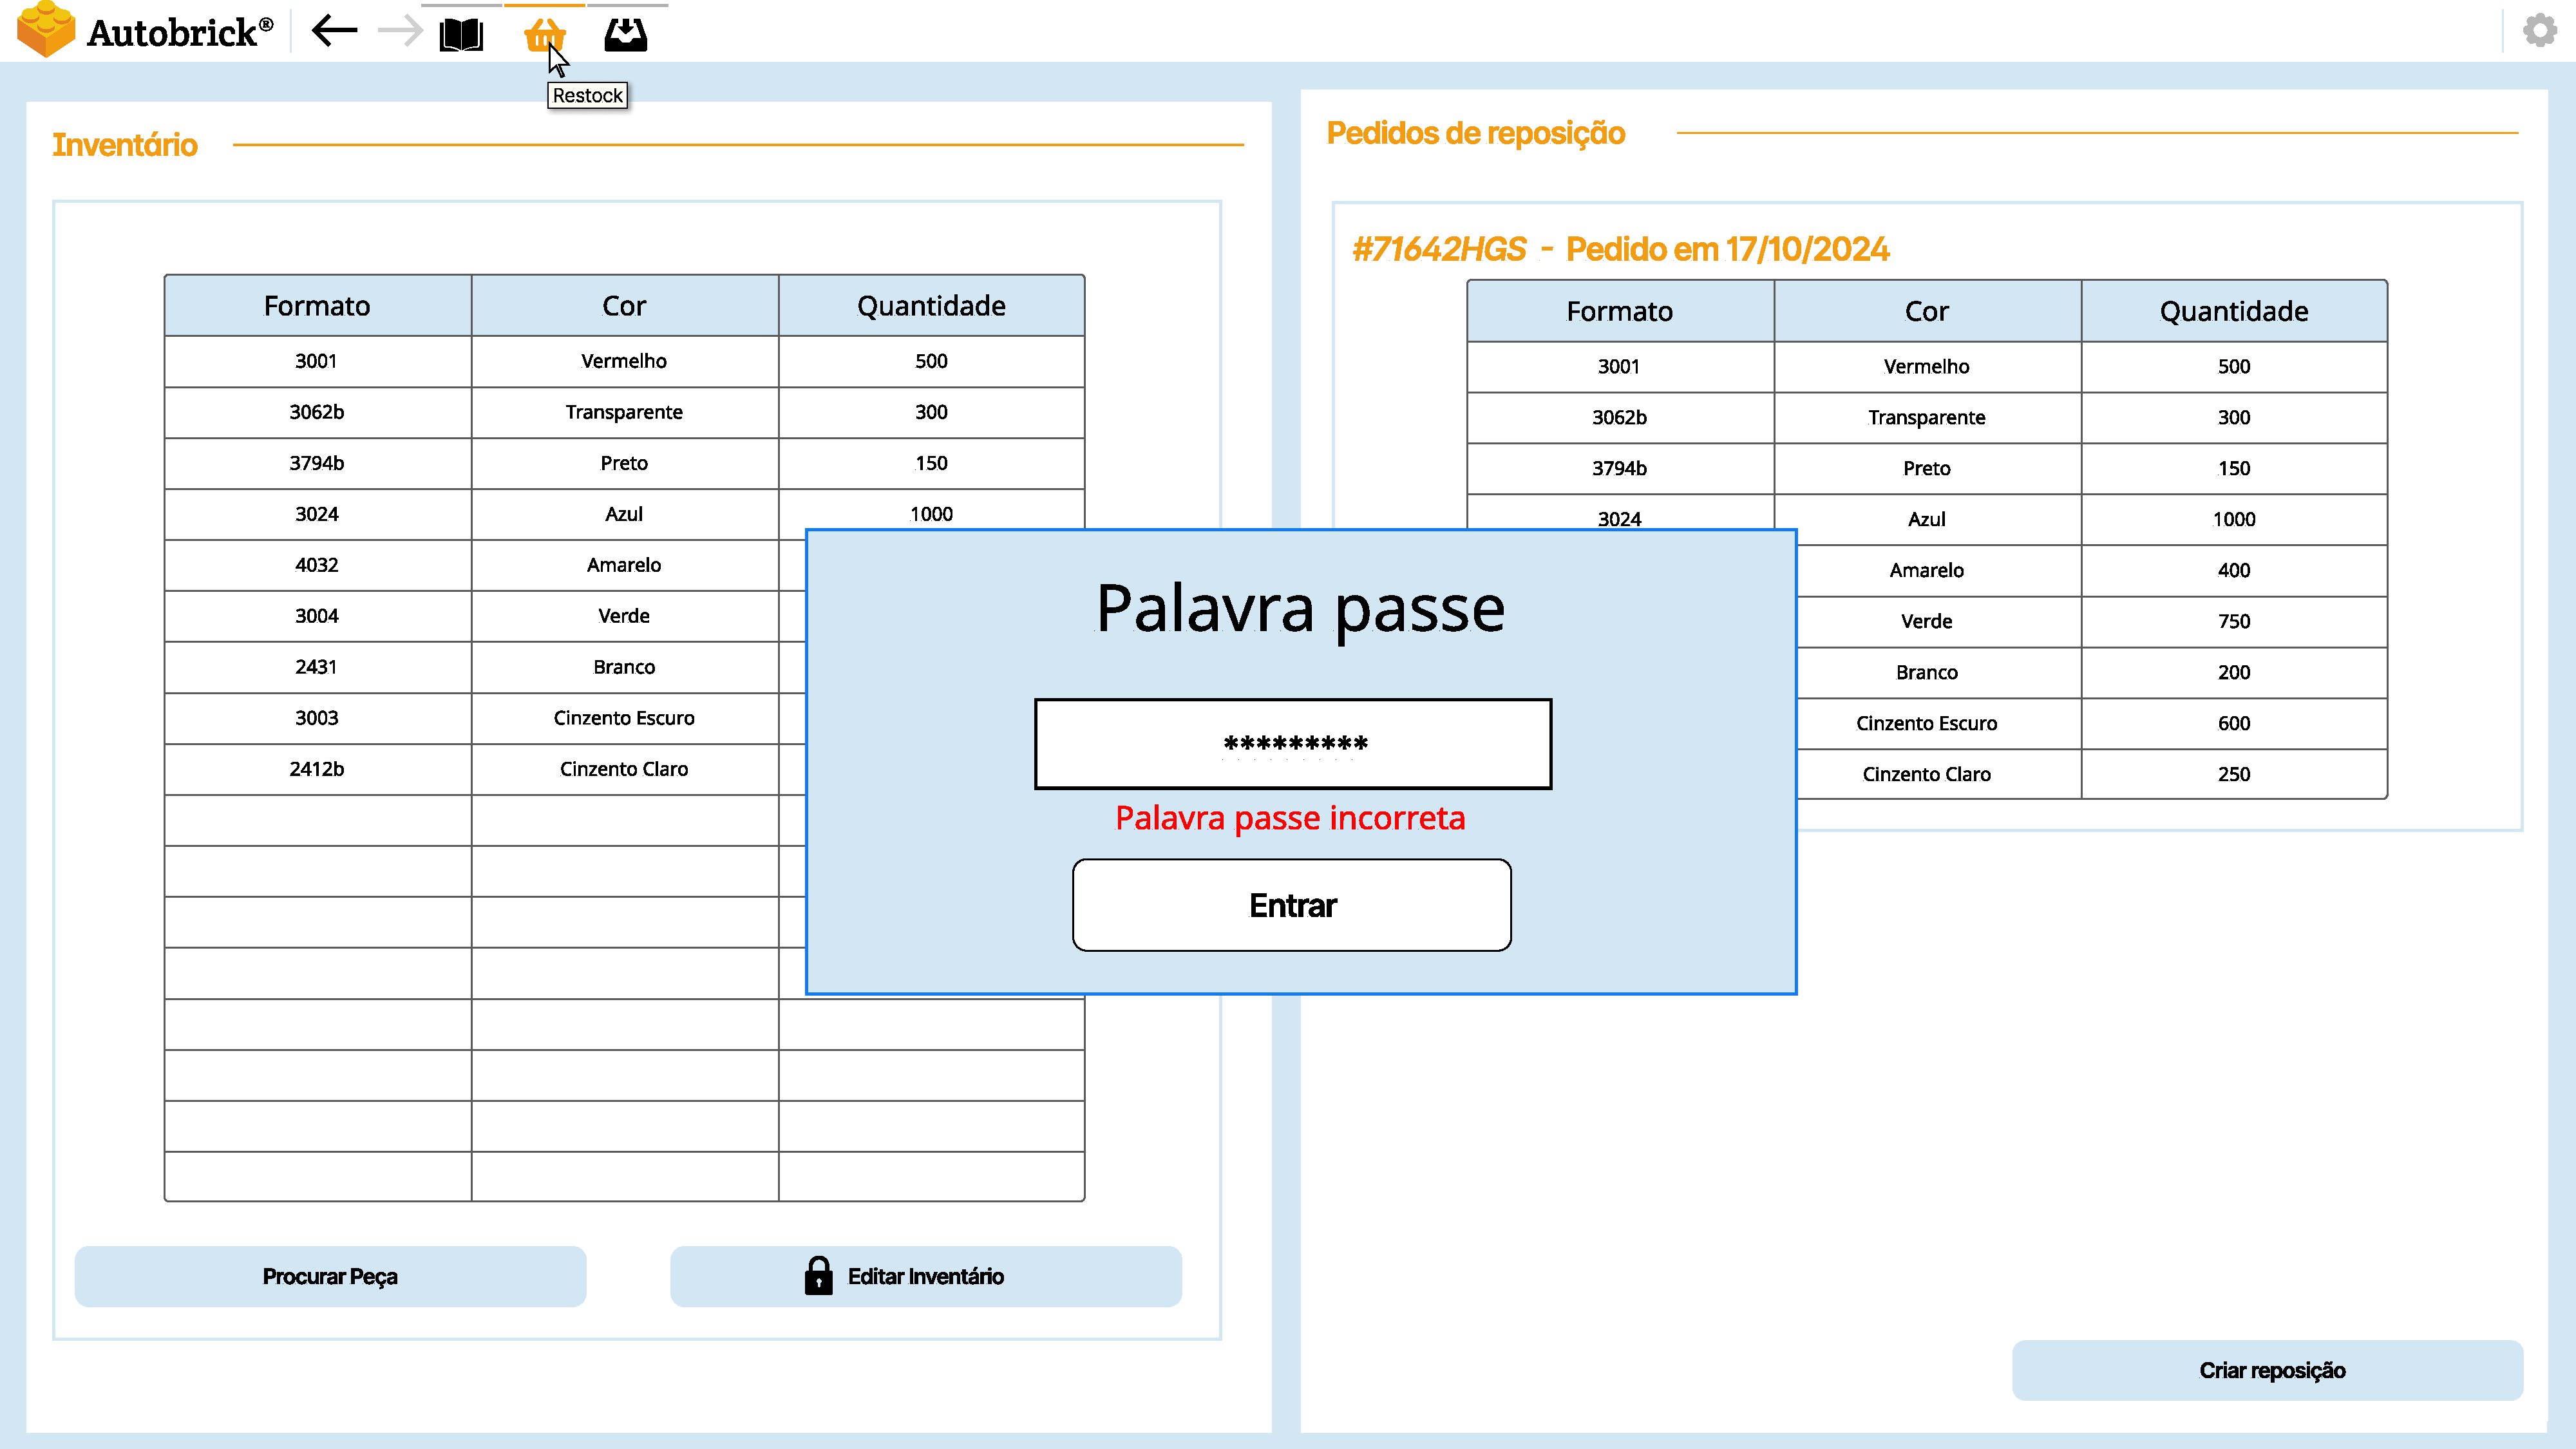
\includegraphics[width=0.99\linewidth, frame]{images/Admin Menu Alteração.pdf}
            \caption{Página de inventário após interação com botão de editar inventário (Palavra passe de administrador errada)}
            \label{fig:EditarInv1}
        \end{figure}
    
        \begin{figure}[h!]
            \centering
            \includegraphics[width=0.99\linewidth, frame]{images/Alterar inventário.pdf}
            \caption{Página de inventário após interação com botão de editar inventário (Após a palavra passe de administrador ser inserida)}
            \label{fig:EditarInv2}
        \end{figure}

        \clearpage    
        \begin{figure}
            \centering
            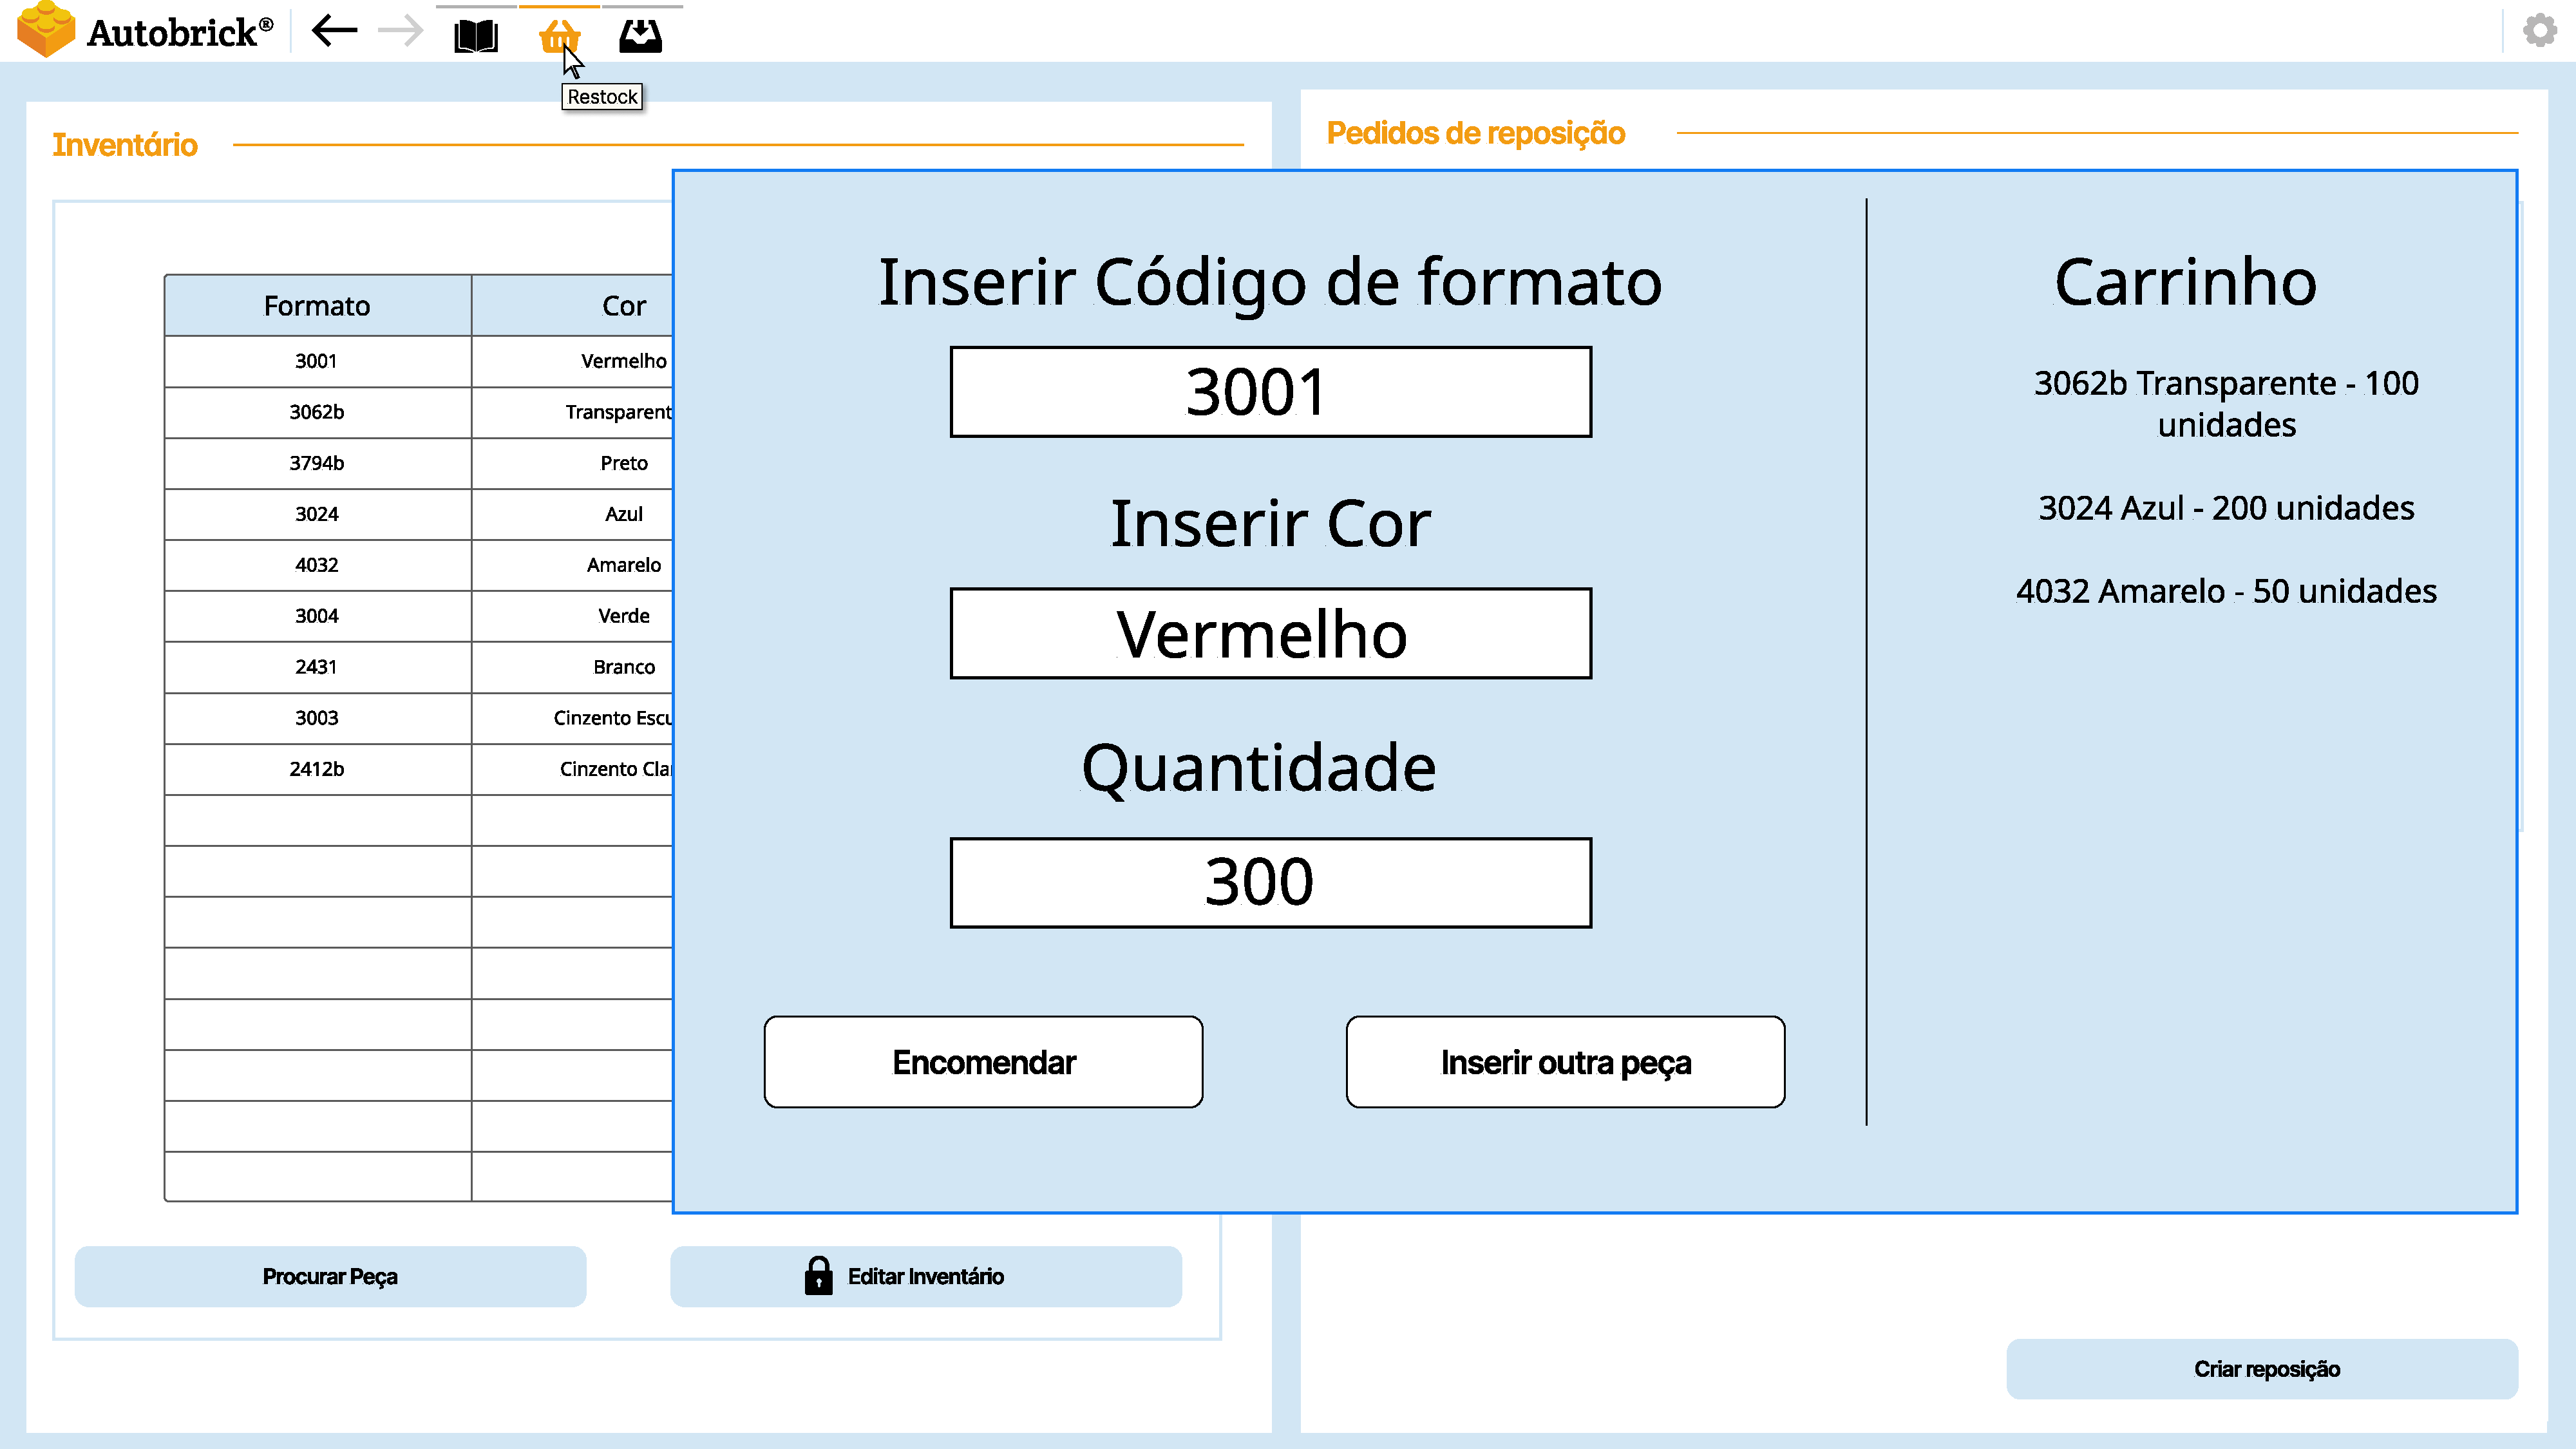
\includegraphics[width=0.99\linewidth, frame]{images/Restock Manual.pdf}
            \caption{Página de inventário após interação com botão de criar reposição}
            \label{fig:Reposição}
        \end{figure}

        \clearpage
        \subsection{Interfaces de Catálogo}
    
        \begin{figure}[ht]
            \centering
            \includegraphics[width=0.99\linewidth, frame]{images/Catálogo.pdf}
            \caption{Página de catálogo}
            \label{fig:Catálogo}
        \end{figure}

    Nesta páina é possível consultar uma lista com todos os modelos disponíveis (ver 3.3.3.1) bem como visualizar o manual de um modelo utilizando o botão "Visualizar Montagem" (ver 3.3.3.2).
    As figuras \ref{fig:Modelo Meio} e \ref{fig:Modelo Fim} mostram a página de instruções de um modelo de exemplo.
    
        \begin{figure}[h!]
            \centering
            \includegraphics[width=0.99\linewidth, frame]{images/Visualizar montagem.pdf}
            \caption{Página de catálogo após interação com botão de visualizar montagem}
            \label{fig:Visualizar modelo}
        \end{figure}
    
        \begin{figure}[h!]
            \centering
            \includegraphics[width=0.99\linewidth, frame]{images/Instructions Manual I.pdf}
            \caption{Página de instruções para modelo (meio da montagem)}
            \label{fig:Modelo Meio}
        \end{figure}
    
        \begin{figure}[h!]
            \centering
            \includegraphics[width=0.99\linewidth, frame]{images/Instructions Manual II.pdf}
            \caption{Página de instruções para modelo (fim da montagem)}
            \label{fig:Modelo Fim}
        \end{figure}
    
%==========================================================================
% END #5 - ESBOÇO DOS INTERFACES DO SISTEMA
%==========================================================================